%!TEX encoding = UTF-8 Unicode
\chapter{动态分析}
动态分析是需要样本中的代码在目标系统实际运行起来的分析方式。与静态分析相比,它能够获得更直观、更全面的结果。此外,对采用了代码混淆等对抗技术的样本,动态分析会是主要的手段。

与静态分析相比,动态分析的知识点比较杂,没有系统的基础知识,也需要更高的创造力和综合能力。

\section{运行环境}
\subsection{模拟器}
Android SDK提供了用于应用软件开发的Android模拟器\lstinline!emulator!\cite{url:android_emulator}\index{emulator},是首选的运行环境。
\begin{figure}[htbp]
  \centering
  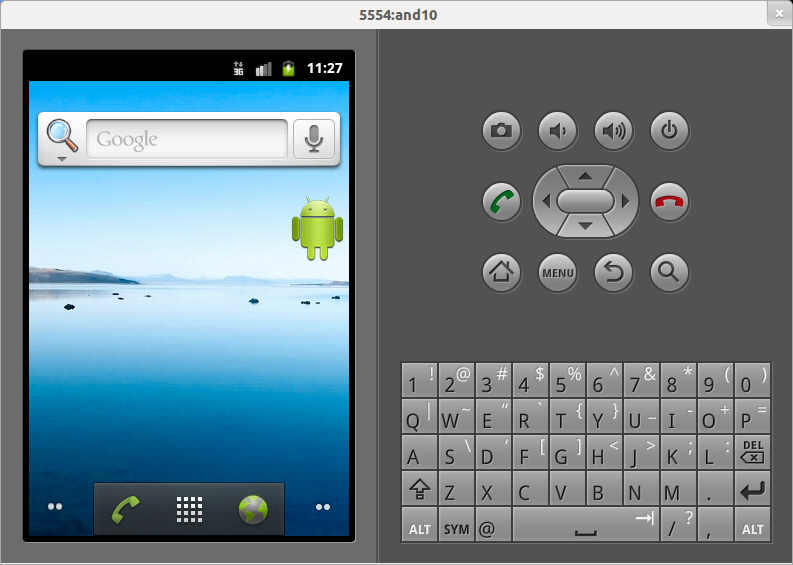
\includegraphics[width=14cm]{image/emulator.png}
  \caption{emulator模拟器}
\end{figure}

\lstinline!emulator!中模拟的Android系称为AVD(Android Virtual Device),由SDK中\lstinline!android!\cite{url:android_android}\index{android}工具创建:
\begin{lstlisting}[language=bash, numbers=none]
 $ android create avd -n my_avd -t android-10
\end{lstlisting}

可以使用图形化的AVD Manager直接启动AVD,也可以使用\lstinline!emulator!直接启动。使用命令行参数可以手工指定一些高级选项,这在一些分析时可能会用上。这些参数如下:
\begin{itemize}
\item \lstinline!-avd!,必选参数,指定AVD的名字
\item \lstinline!-data!,手工指定一个data分区镜像文件
\item \lstinline!-ramdisk!,手工指定一个RAM镜像文件
\item \lstinline!-kernel!,手工指定一个内核文件
\item \lstinline!-system!,手工指定一个system分区镜像文件
\item \lstinline!-sdcard!,手工指定一个SD卡镜像文件,该文件可以用\lstinline!mksdcard!创建
\item \lstinline!-dns-server!,给出DNS服务器地址,可以指向自己搭建的DNS服务器,模拟样本依赖的服务器
\item \lstinline!-http-proxy!,当样本访问被墙的网址时,可以通过SSH隧道和本地HTTP端口转发
\item \lstinline!-debug!,打开或关闭指定的调试标签,让\lstinline!emulator!输出调试信息,可以使用\lstinline!emulator -help-debug-tags!察看有哪些标签
\end{itemize}
例如,\lstinline!droidbox!的启动命令行是:
\begin{lstlisting}[language=bash, numbers=none]
 $ emulator -avd droidbox -system system.img -ramdisk ramdisk.img -kernel zImage -prop dalvik.vm.execution-mode=int:portable
\end{lstlisting}

\lstinline!emulator!的不足之处是:
\begin{itemize}
\item 虽然可以模拟短信和通话,但并没有与真正的移动通信网络相连
\item 对依赖于ROM环境、依赖于特定手机型号的样本不起作用
\end{itemize}

\subsection{手机}
手机可以提供运行样本的真实环境,并且与移动通信网相连。主要缺点是成本较高。

推荐Google的Nexus S型号手机,原因包括:
\begin{itemize}
  \item 直接使用Android源码可以编译Nexus S系统镜像,自行修改的源码可以获得真实的运行环境,并且可以对该镜像做自由的修改,比如有root权限、可以修改启动配置等
  \item 诸如TaintDroid、AppFence等项目均提供了用于Nexus S的源码
  \item 可以在第一时间获得新版本系统,例如Android 4.0
  \item 综合性价比较高
\end{itemize}

\subsection{Android-x86}
Android-x86\cite{url:android_x86}\index{Android-x86}提供了用于Intel x86处理器的Android系统镜像,可以将其安装到诸如VirtualBox和VMware WorkStation这样的虚拟机中。有研究称该项目系统的启动速度是\lstinline!emulator!中AVD启动速度的四分之一。

\section{设备管理}
\subsection{adb}
\lstinline!adb!是连接PC与设备(模拟器或手机)的主要工具,其用法在Android开发文档中有详细的说明\cite{url:android_adb}。

它的功能包括:
\begin{itemize}
\item 提供了一个访问Android底层Linux系统的shell
\item 通过push和pull在PC和设备之间传输文件
\item 通过install和uninstall安装或卸载应用程序
\item 转发对Android系统的调试指令和数据
\item 通过logcat获取系统进程和应用程序输出的日志信息
\end{itemize}

\subsubsection{shell}
输入下面的命令将连接设备并打开一个shell。
\begin{lstlisting}[numbers=none]
 $ adb shell
\end{lstlisting}
如果得到的提示符是\lstinline!\$!,是一个没有root权限的shell;如果提示符是\lstinline!\#!,则是有root权限的shell。

在设备系统的/system/bin目录下,提供了一些实用工具,例如Linux下常用的\lstinline!ls!、\lstinline!chmod!等,也有一些Android的小工具,例如\lstinline!am!等。

如果只是执行一两条指令,可以不进入交互式shell,而直接在本地完成,例如:
\begin{lstlisting}[numbers=none]
 $ adb shell ls /data/data
\end{lstlisting}

shell是在Linux层操作Android系统的主要方式。

\subsubsection{文件传输}
把本地文件发送至设备路径:
\begin{lstlisting}[numbers=none]
 $ adb push /path/to/local/file /path/to/device/target
\end{lstlisting}

从设备的指定路径获取文件:
\begin{lstlisting}[numbers=none]
 $ adb pull /path/to/device/file /path/to/local/target
\end{lstlisting}
这两条命令需要对设备端的路径和文件有相应的写和读的权限。如果权限不够,需要在root权限的shell下\lstinline!remount!分区;或者使用\lstinline!/data/local/tmp!目录作为中转站(普通权限的shell即可访问该目录),在root权限下做进一步拷贝。例如:
\begin{lstlisting}[numbers=none]
 host$ adb push ./tcpdump /data/local/tmp
 host$ adb shell
 device$ su
 device# cp /data/local/tmp/tcpdump /system/bin/tcpdump
 device# chmod 6755 /system/bin/tcpdump
 device# exit
 device$ exit
 host$
\end{lstlisting}

\subsubsection{安装和卸载}
将本地APK文件安装至设备很简单:
\begin{lstlisting}[numbers=none]
 $ adb install /path/to/local/app.apk
\end{lstlisting}

而与之相应的卸载则需要先知道应用程序的package name:
\begin{lstlisting}[language=bash, numbers=none]
 $ adb uninstall app.full.package.name
\end{lstlisting}
这个package name与该应用在设备系统的\lstinline!/data/data!路径下的子目录名完全相同。

\subsubsection{转发端口}
例如建立本地端口6100与设备端口7100之间的转发:
\begin{lstlisting}[numbers=none]
 $ adb forward tcp:6100 tcp:7100
\end{lstlisting}
这种转发将在后面的远程调试时使用。

\subsubsection{捕获日志}
使用:
\begin{lstlisting}[numbers=none]
 $ adb logcat
\end{lstlisting}
可以在本地终端显示应用程序的运行日志,例如调试信息和出错信息等。\lstinline!logcat!可以配合参数与日志过滤器,例如\lstinline!droidbox!的日志捕获使用的命令就是:
\begin{lstlisting}[numbers=none]
 $ adb logcat dalvikvm:W *:S
\end{lstlisting}
具体用法可以参考\lstinline!adb!的文档。

\subsection{ddms}
\begin{figure}[htbp]
  \centering
  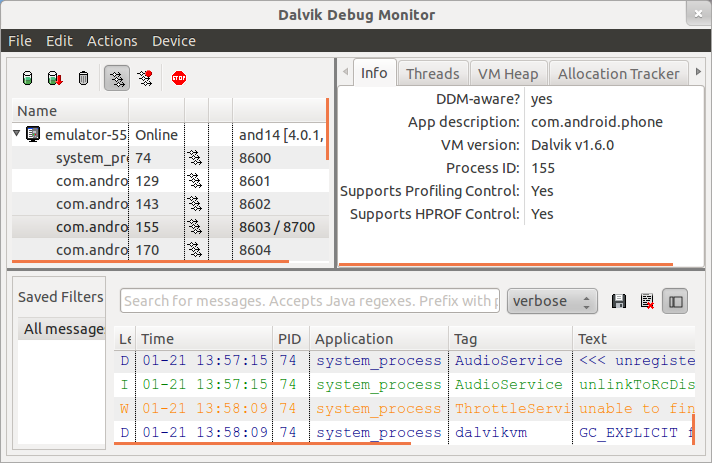
\includegraphics[width=14cm]{image/ddms.png}
  \caption{ddms的主界面}
\end{figure}
SDK中的\lstinline!ddms!\index{ddms}工具提供了一个可视化调试环境,功能包括:
\begin{itemize}
  \item 设备进程和线程管理
  \item 进程的内存管理
  \item 可视化logcat工具,以及图形化的过滤器
  \item 设备文件浏览
  \item 设备屏幕捕获
  \item dump设备状态和应用程序状态
\end{itemize}

\section{网络分析}
\subsection{tcpdump}
为了捕获样本在运行期间产生的网络数据,需要对其抓包。主要工具是\lstinline!tcpdump!\index{tcpdump}。针对不同的场景,可以在三个不同的位置使用这一工具。

\subsubsection{模拟器}
模拟器\lstinline!emulator!有一个没有公开的参数\lstinline!-tcpdump!,在启动模拟器时,通过该参数指定一个本地文件路径,可以将模拟器运行期间产生的所有网络数据捕获到指定的文件,该文件为PCAP格式,可以使用\lstinline!wireshark!或\lstinline!libpcap!解析。
\begin{lstlisting}[numbers=none]
 $ emulator -avd my_avd_name -tcpdump /path/to/dump.pcap
\end{lstlisting}
使用模拟器抓包的优点是不会捕获到本机其他进程产生的网络数据,缺点是:
\begin{itemize}
  \item 对真实手机显然无效
  \item Android系统在开机时大量使用网络端口传输调试信息等,因此捕获的PCAP数据包中有大量的无意义数据需要区分
\end{itemize}

\subsubsection{Android系统}
有移植到Android底层的原生\lstinline!tcpdump!工具,但其运行需要root权限。这一工具可以在模拟器中的系统里运行,但更多时候用于真实手机系统的抓包。
\begin{lstlisting}[numbers=none]
 host$ adb push ./tcpdump /data/local/tmp/tcpdump
 host$ adb shell
 device$ su
 device# chmod 6755 /data/local/tmp/tcpdump
 device# /data/local/tmp/tcpdump -p -vv -s 0 -w /sdcard/capture.pcap
\end{lstlisting}
其中,最后一行是启动\lstinline!tcpdump!,捕获一切数据包并保存在SD卡根目录下。不再需要捕包时,可以按下Ctrl + C终止。

在系统中使用原生\lstinline!tcpdump!的优点是能根据需要开始和结束捕包,并且在真实手机上也行之有效。主要缺点是要求拥有系统的root权限。

\subsubsection{Wi-Fi}
如果是没有root权限的手机,接下来的方法就只有通过Wi-Fi接入互联网,并且在网络上捕包了。例如,在无线路由器与网关之间加入一个集线器,在集线器上另外接一根网线到PC机上。由于集线器这种物理层设备会广播所有的网络流量,因此在PC上就可以捕获到手机通过无线路由器与Internet通信的所有数据。这种方案依然存在不足:
\begin{itemize}
  \item 会捕获到所有经过路由器的流量数据
  \item 极少数恶意代码只通过GPRS和3G联网
\end{itemize}

\subsection{Wireshark}
Wireshark\cite{url:wireshark}\index{Wireshark}是分析网络数据最常用也最强大的工具。在此不再专门介绍。

\section{行为模拟}
很多样本的恶意行为只在一定条件下触发,但在分析环境中,这些条件不一定能立即实现。此时需要对相应的条件进行模拟。在Android SDK文档中对此已经有一些介绍\cite{url:android_using_emulator}。

\subsection{am}
\lstinline!am!\index{am}是Android系统中的一个工具,位于/system/bin目录下,实际上是基于\lstinline!/system/framework/am.jar!执行\lstinline!com.android.commands.am.Am!类的代码。\lstinline!am!的主要作用即是启动活动(activity)、意图(intent)、广播(broadcast)等。

\lstinline!am!的用法如下:
\lstinputlisting[firstline=1, lastline=20, numbers=none]{code/am.txt}

其中,\lstinline!am start!用于启动一个活动;\lstinline!am startservice!用于启动一个服务;\lstinline!am broadcast!用于发送一个广播。它们的参数都是一个一个意图(Intent)。\lstinline!am!中intent的写法如下:
\lstinputlisting[firstline=76, lastline=101, numbers=none]{code/am.txt}

\subsection{telnet}

\subsection{DNS}

\subsection{openBTS}

\section{行为跟踪}
\subsection{LBE}
\subsection{androidAuditTools}
androidAuditTools\cite{url:androidaudittools}

\section{调试}
\label{Sec:debug}
\subsection{apktool}
\subsection{AndBug}

\section{沙盒}
\subsection{TaintDroid}
\subsection{droidbox}
\subsection{Anubis}

\section{衍生文件}
